%%%%%%%%%%%%%%%%%%%%%%%%%%%%%%%%%%%%%%%%%%%%%%%%%%%%%%%%%%%%%%%%%%%%%%%%%%%%%%%%
%https://www.linkedin.com/in/zachary-neveu	Latex Notes Template
%	Zach Neveu
%	zachary.neveu@gmail.com
%%%%%%%%%%%%%%%%%%%%%%%%%%%%%%%%%%%%%%%%%%%%%%%%%%%%%%%%%%%%%%%%%%%%%%%%%%%%%%%%

% Geometry, font
\documentclass[12pt, letter]{article}
\usepackage[margin=0.8in]{geometry}
\usepackage[T1]{fontenc}
\usepackage{fourier}
\usepackage{titling}
\setlength{\droptitle}{-5em} 
\usepackage[parfill]{parskip}
\usepackage{graphicx}
\graphicspath{{imgs/}}
\usepackage{hyperref}

% Math stuff
\usepackage{amssymb}
\usepackage{amsmath}
\usepackage{bm}

%acronyms
\usepackage{acronym}


% Code Highlighting
\usepackage{minted}
\usemintedstyle{solarizedlight}

\usepackage{booktabs}

\author{Zach Neveu}
\title{ Homework 1 }

\begin{document}
\maketitle

\begin{enumerate}
	\item Problem 1
\begin{minted}{Python}
def divide_by_three(integerlist):
  """
  This function outputs a list where, if the integer on
  the input list is divisible by three, the corresponding
  output is 1 else the output is 0
  """
  return [integerlist[i]%3 == 0 for i in range(len(integerlist))]
\end{minted}

	\item Problem 2: full adder
	\begin{table}[htpb]
		\centering
		\caption{Truth table of full adder}
		\label{tab:truth_table}
		\begin{tabular}{lllll}
		\toprule
		Input 0 & Input 1 & $C_{in}$ & Sum & Carry \\
		\midrule
		0 & 0 & 0 & 0 & 0 \\
		\midrule
		0 & 0 & 1 & 1 & 0 \\
		\midrule
		0 & 1 & 0 & 1 & 0 \\
		\midrule
		0 & 1 & 1 & 0 & 1 \\
		\midrule
		1 & 0 & 0 & 1 & 0 \\
		\midrule
		1 & 0 & 1 & 0 & 1 \\
		\midrule
		1 & 1 & 0 & 0 & 1 \\
		\midrule
		1 & 1 & 1 & 1 & 1 \\
		\bottomrule	
		\end{tabular}
	\end{table}

\begin{figure}[H]
	\centering
	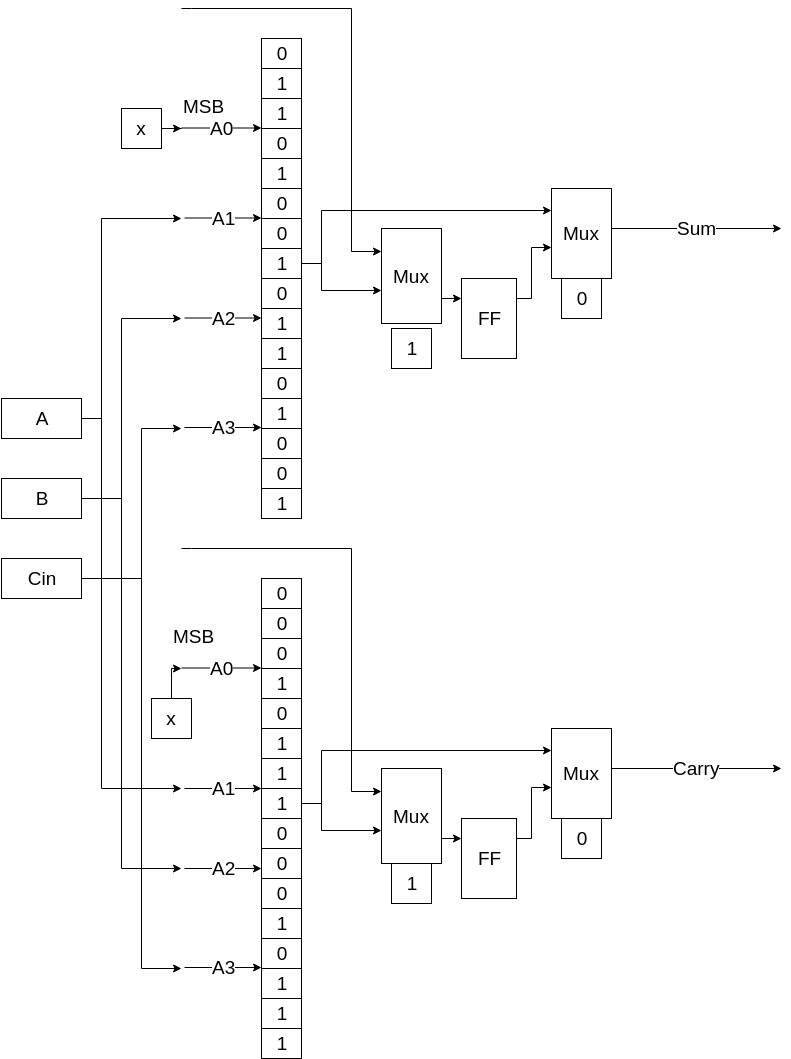
\includegraphics[width=0.8\textwidth]{full_adder}
	\caption{Full Adder on Simplified Logic Slices}
	\label{fig:full_adder}
\end{figure}

	\item Problem 3: "101" Detector
	\begin{figure}[h]
		\centering
		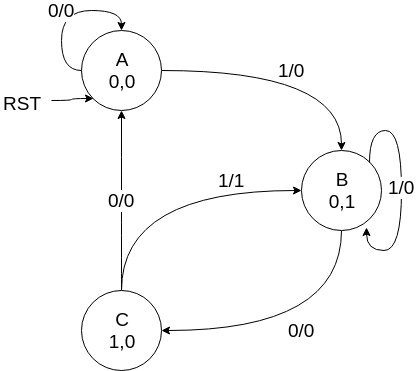
\includegraphics[width=0.5\textwidth]{101_sm}
		\caption{State machine for "101" detector}
		\label{fig:101_sm}
	\end{figure}

	\begin{table}[h]
		\centering
		\caption{States to binary for "101" recognizer}
		\label{tab:label}
		\begin{tabular}{ll}
		State & Binary Representation \\
		\toprule
		A & "00" \\
		\midrule
		B & "01" \\
		\midrule
		C & "10" \\
		\botomrule
		\end{tabular}
	\end{table}

	\begin{table}[h]
		\centering
		\caption{Truth Table for State and Output of "101" detector}
		\label{tab:label}
		\begin{tabular}{llll|lll}
		Q & A & Q_0 & Q_1 & Q_0^* & Q_1^* & Output \\
		\toprule
		A & 0 & 0 & 0 & 0 & 0 & 0 \\
		\midrule
		B & 0 & 0 & 1 & 1 & 0 & 0 \\
		\midrule
		C & 0 & 1 & 0 & 0 & 0 & 0 \\
		\midrule
		n/a & 0 & 1 & 1 & x & x & x \\
		\midrule
		A & 1 & 0 & 0 & 0 & 1 & 0 \\
		\midrule
		B & 1 & 0 & 1 & 0 & 1 & 0 \\
		\midrule
		C & 1 & 1 & 0 & 0 & 1 & 1 \\
		\midrule
		n/a & 1 & 1 & 1 & x & x & x \\
		\end{tabular}
	\end{table}

	\begin{figure}[h]
		\begin{equation}
		\begin{align*}
			Q_0^{*} = \overline{x} \land \overline{Q_0} \\
			Q_1^{*} = x \\
			Output = x \land Q_0
	   .\end{align*}
		\end{equation}
		\caption{Equations for State and Output of "101" detector}
		\label{fig:}
	\end{figure}

	\begin{figure}[h]
		\centering
		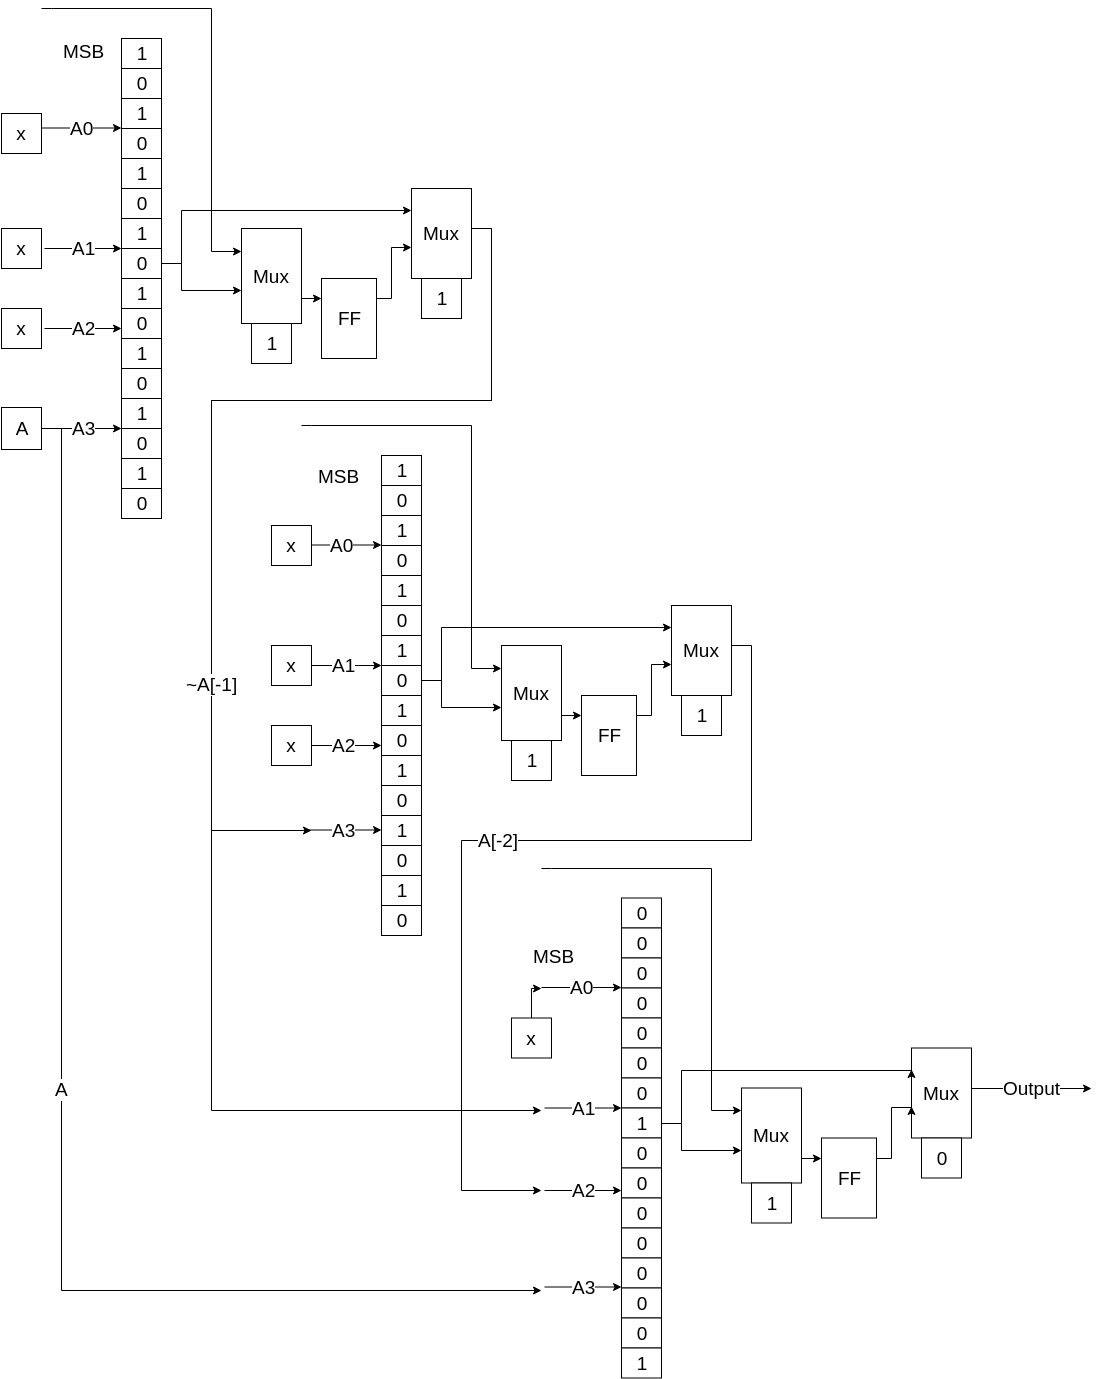
\includegraphics[width=0.8\textwidth]{101_slices.png}
		\caption{"101" recognizer implemented on simplified logic slices}
		\label{fig:101_slices-png}
	\end{figure}
\end{enumerate}
\end{document}
